%!TEX root = ../Main.tex

\section{Methodology and Data}\label{sec:4MethodData}

\subsection{Data and Calculation of Input Factors}\label{sec:41Data}
The data used in this study are from several sources. The realized variance of the S\&P 500 index is obtained from the \textcite{Oxford:RV}. Daily VIX values are the closing values from \gls{CBOE}. As after September 22, 2003 \gls{CBOE} started to use a revised methodology for the VIX, the prices had to be calculated ex post, thus the data was taken from \textcite{CBOE:old} and \textcite{CBOE:new}. The S\&P 500 which is only used for visualisation is also taken from \gls{CBOE} under \textcite{SandP}. The sample consists of daily data in the period from January 2000 to December 2017. \\
The calculation of the daily realized variance is calculated by \textcite{Oxford:RV} as the sum of squared high-frequency returns, as explained in \ref{sec:221RV}. The formula is given by 
\begin{align}
\sigma_{t} = sum x_{t}^{2}
\end{align}
with $x_{t} = X_{t} - X_{t-1}$ and $X_{t}$ the logarithm of the price at time $t$.  There are many advantages of using high-frequency returns, textcite{andersen2003} for example point out that they help both for predicting again high-frequency returns, but also that they contain information for longer horizons, such as monthly or quarterly. In this case, 5-min index returns were used. The data is cleaned by \textcite{Oxford:RV} in four ways. First, entries outside the timestamp when exchanges are open are deleted. Secondly, entries with the same time stamp are replaced with the median bid-ask price. Thirdly entries with a negative spread (as they violate the no-arbitrage condition) or extremely large spread (50 times the median of the day) are deleted. Lastly, entries for which the mid-quote deviated largely from the mean where deleted. To derive the realized volatility, the square root of the realized variance is taken:
\begin{align}
RV_{t} = sqrt(sum x_{t}^{2}).
\end{align}
The monthly averages of the realized volatility used in the HAR-RV model are the rolling averages over the respective time periods. As in \textcite{corsi2009} the periods included are daily, weekly(average over 5 days) and monthly (average over 22 days).  \\
For the VIX the daily closing value is taken, as it contains the information from the whole day. The calculation is described in \ref{sec:223VIX}. To display the data in a more intuitive manner, the annualized VIX is divided by the square root of 252 as in \textcite{blair2000} and \textcite{whaley2008}, to get the daily data.\\
The S\&P 500 together with the VIX is illustrated in \ref{fig1} and the realized vola is added in \ref{fig2}. It can be seen that both the realized volatility and the VIX are particularly high during the period of the crisis between 2008 and 2012. To account for this period, a dummy was included in the model.

%\begin{figure}[!htbp]\label{fig1}
%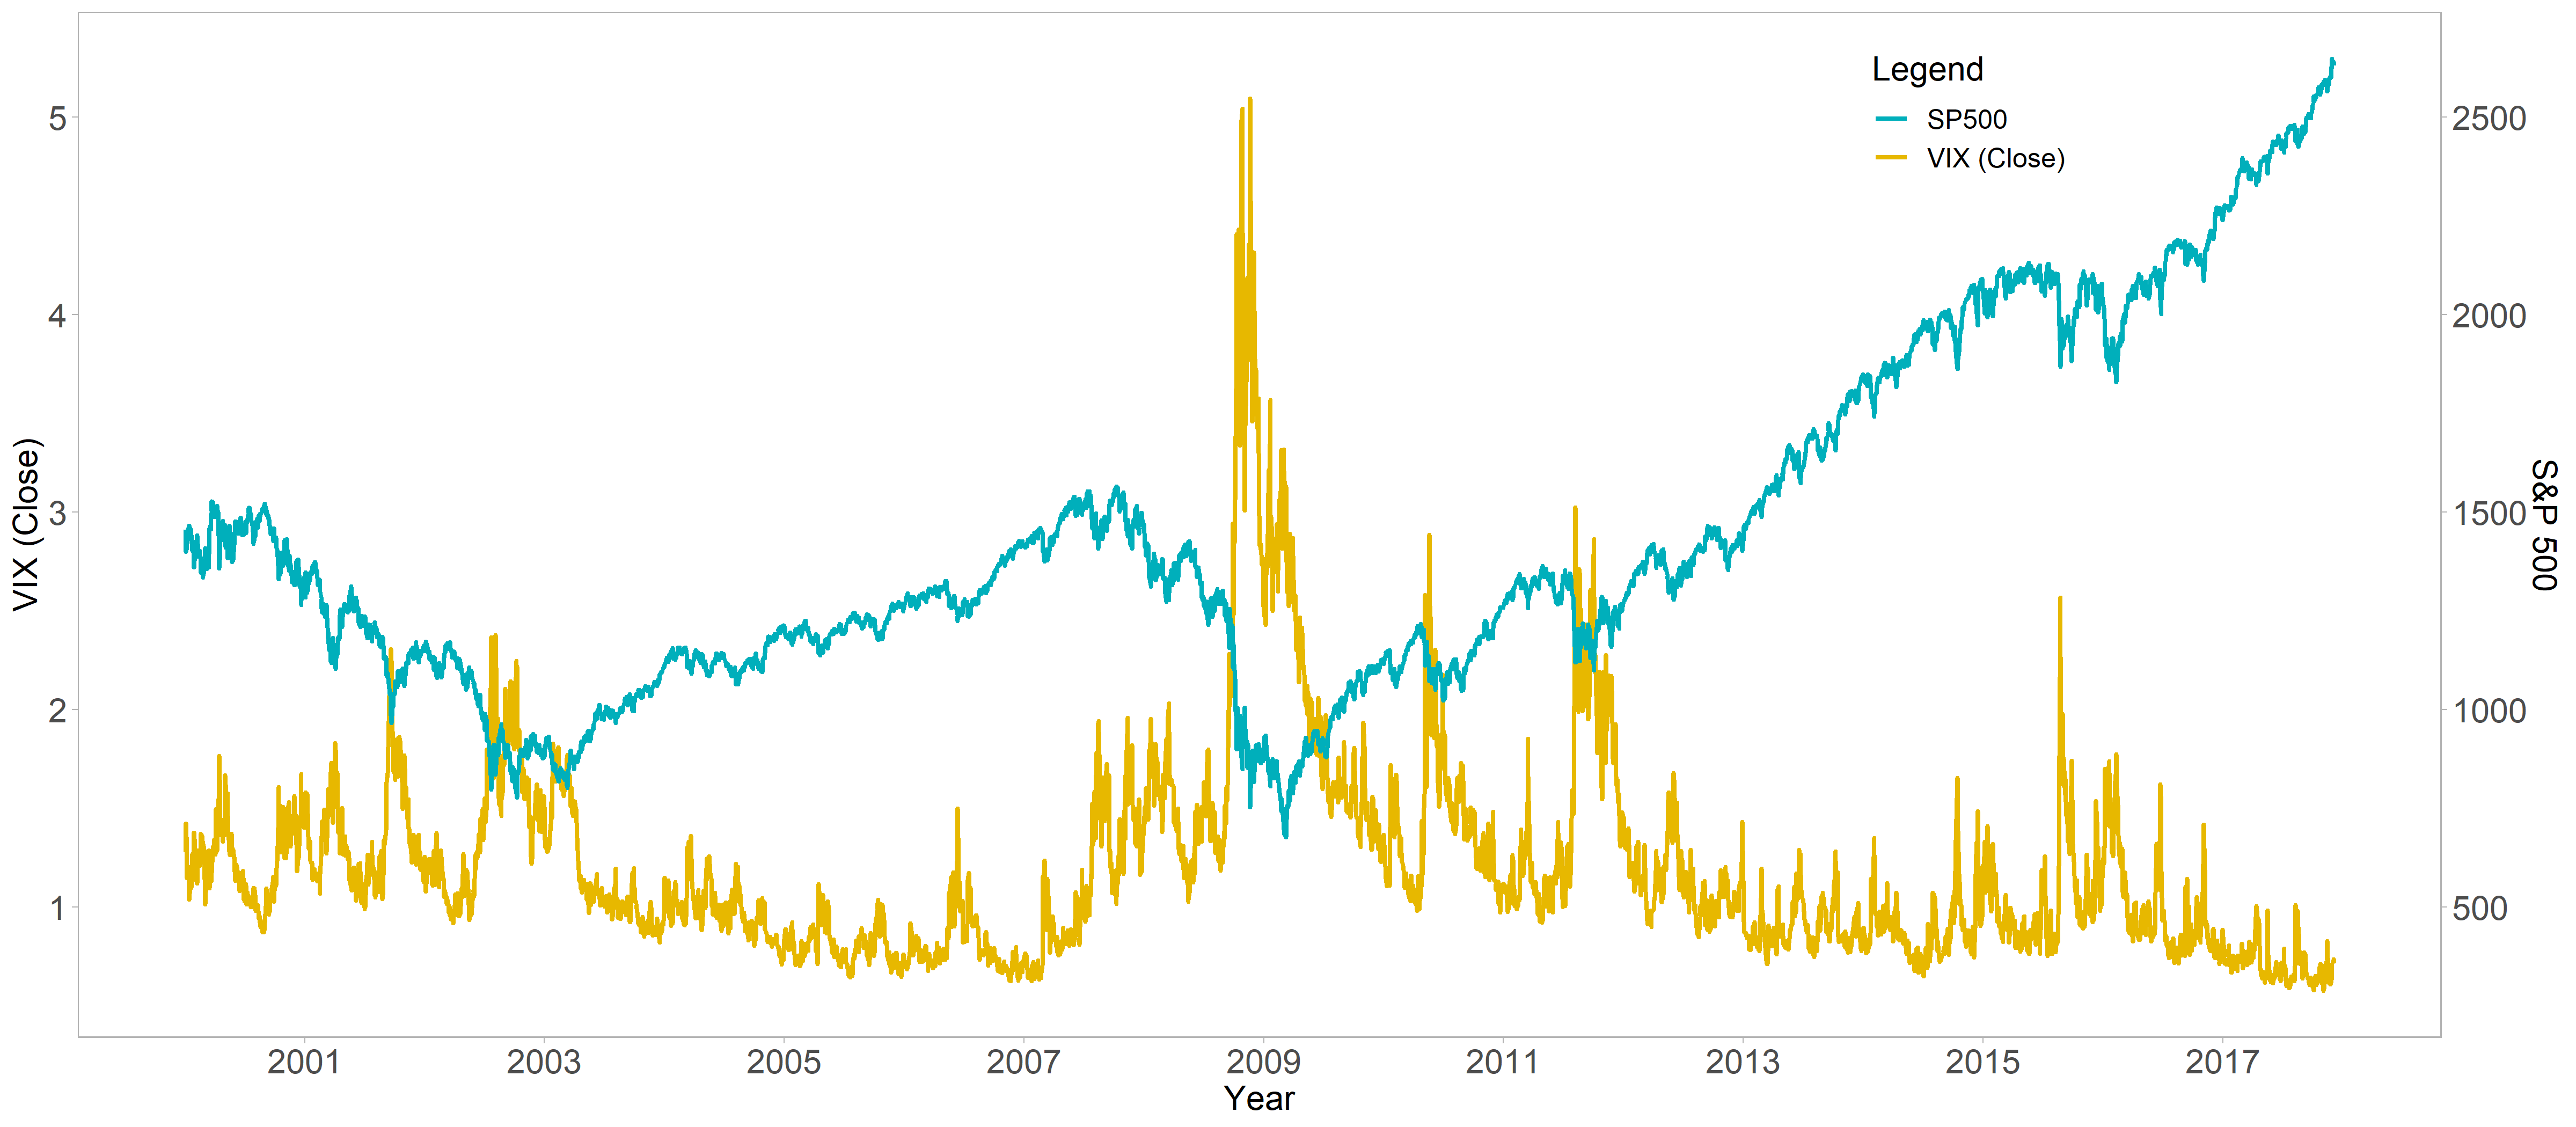
\includegraphics[width=16cm, height=8cm]{pictures/SPandViX.png}
%\end{figure}

%\begin{figure}[!htbp]\label{fig2}
%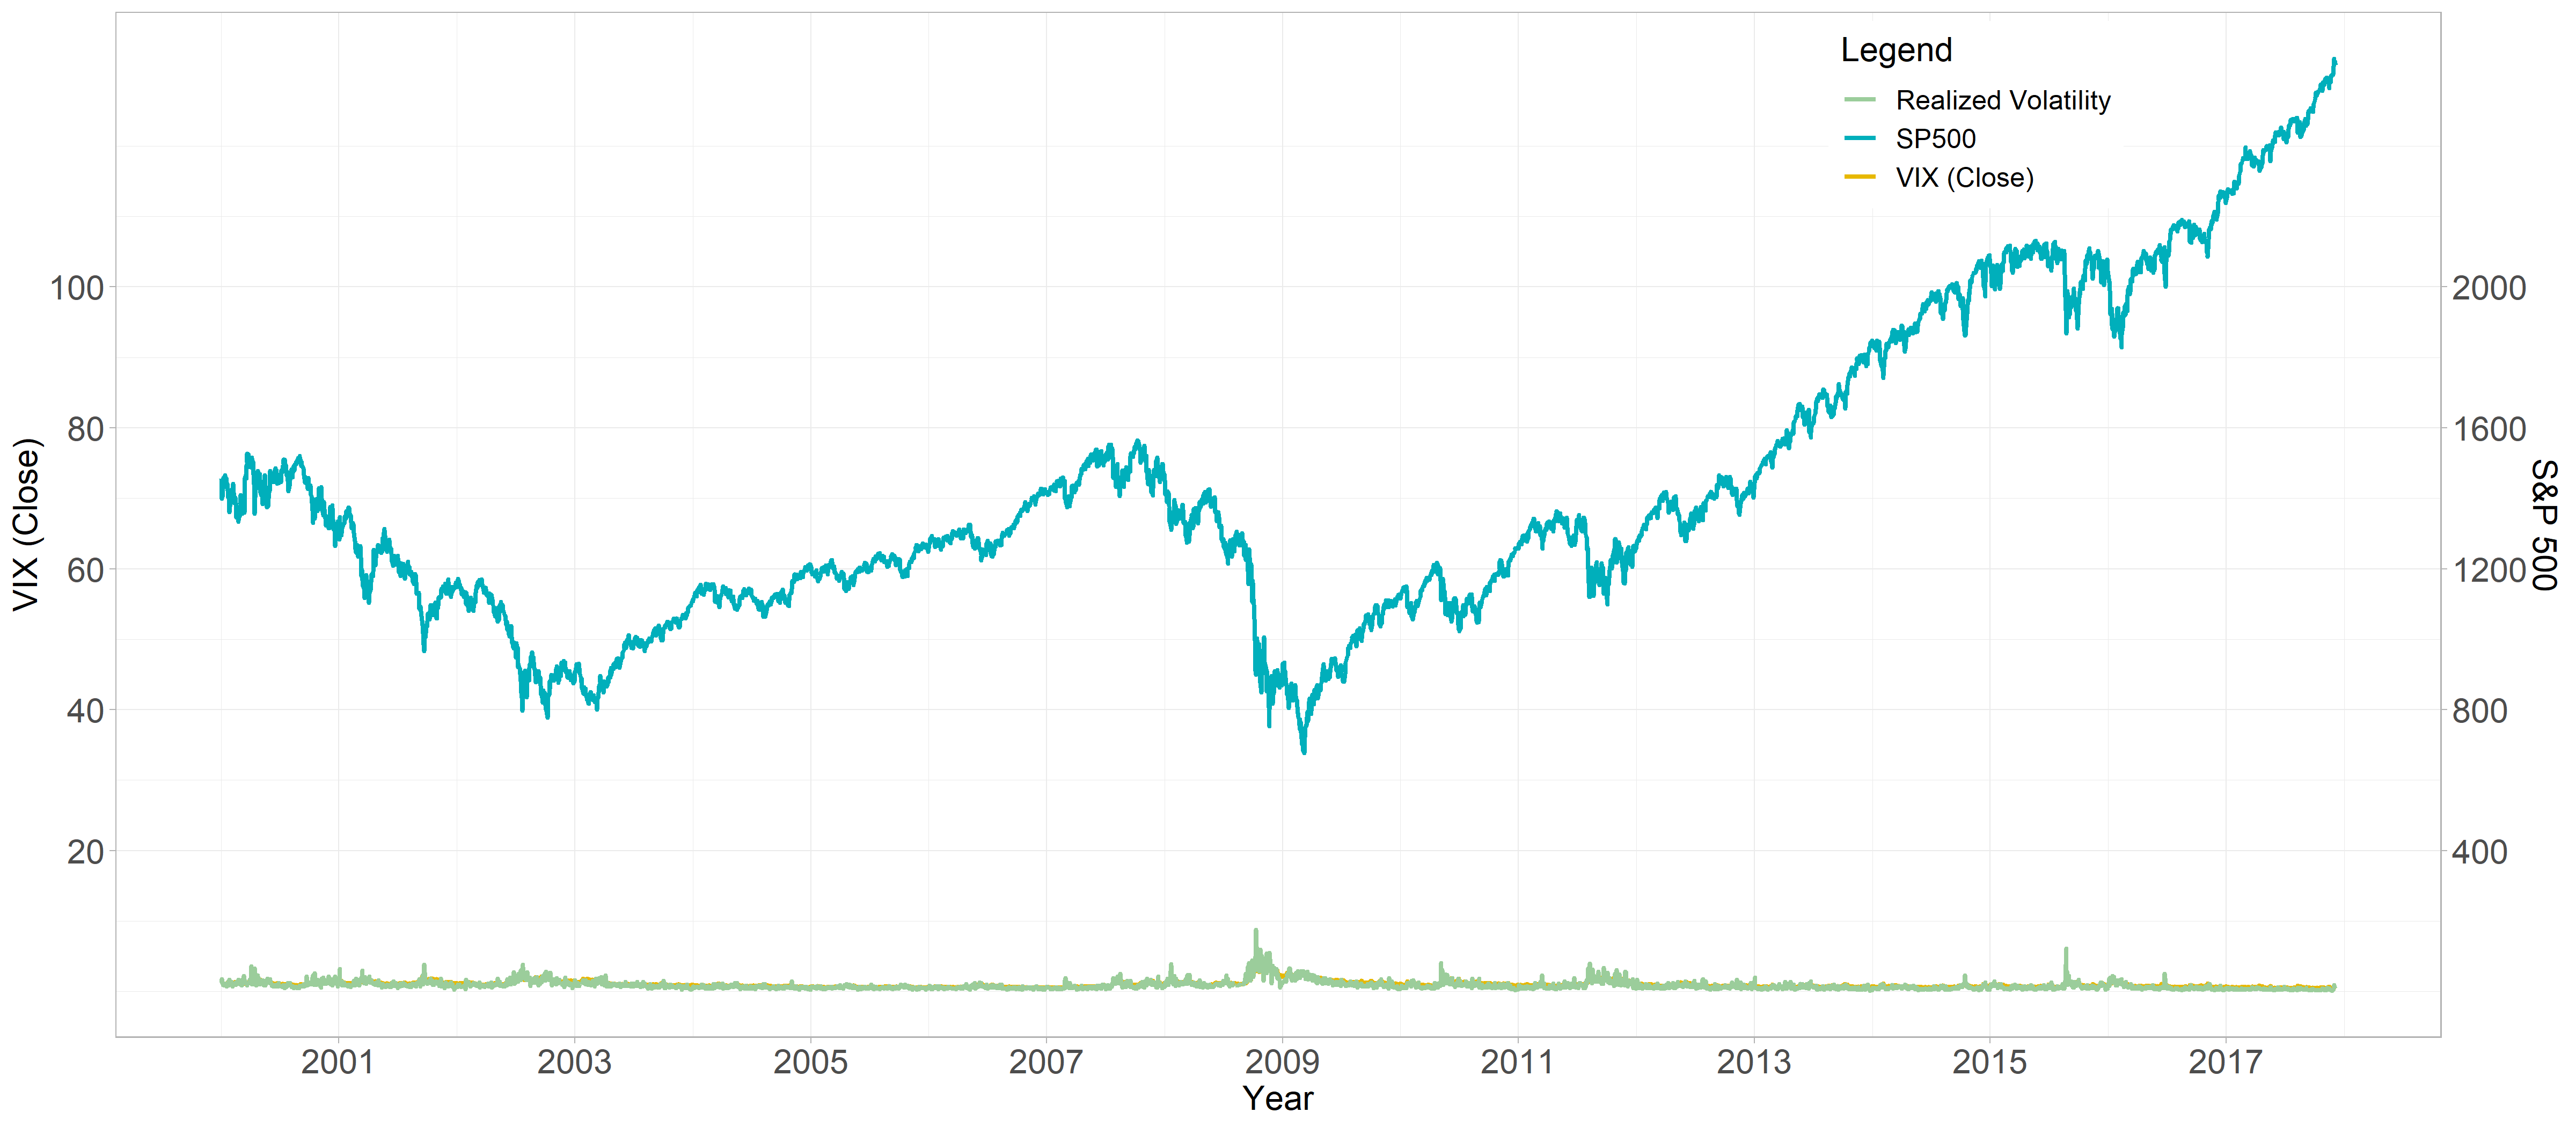
\includegraphics[width=16cm, height=8cm]{pictures/SPandVolandViX.png}
%\end{figure}

add: Data from \citeauthor{heber2009}



\subsection{Methodology: Linear Regression and HAR-RV model}\label{sec:42Method}
Consistent with prior research, for example \textcite{jiang2003}, \textcite{canina1993} or \textcite{christensen1998}, both univariate and encompassing regression analysis is used to analyse the information content of volatility measures. In the univariate regression, the realized volatility is only regressed on the historic data. For comparison, realized volatility is regressed on both historic data and the VIX in the encompassing regression analysis. Thus the encompassing regression analysis gives information about the relative importance of the volatility measures, and whether the VIX as one of them subsumes the information from the historic volatility. The two regressions are then given by:
\begin{align}\label{eq:myregression}
RV_{t+1d} = c + \beta^{d} RV^{d}_{t} + \beta^{w} RV^{w}_{t} + \beta^{m} RV^{m}_{t}  \\
RV_{t+1d} = c + \beta^{d} RV^{d}_{t} + \beta^{w} RV^{w}_{t} + \beta^{m} RV^{m}_{t} + \beta^{VIX} VIX
\end{align}
with .. (explain variables again?). In alignment with \textcite{corsi2009}, the Newey-West covariance correction is used, to account for the possible presence of serial correlation in the data, as serial correlation causes both the Gauss-Markow and Classical linear model assumptions to fail. 


\subsection{Limitations}\label{sec:32Limits}
As volatility is stochastic, the ex-ante estimation will not equal the return volatility, as it is a measurement over an aggregated discrete time period \parencite{andersen2001}.
The VIX might be flawed, as \textcite{jiang2007} showed.
